\begin{frame}{Progress Is Fastest Where Answers Can Be Checked}
\begin{columns}[c]
\column{0.4\textwidth}
\centering
\begin{tikzpicture}[box/.style={draw, rounded corners, align=center, minimum height=1.1cm, minimum width=3.4cm}, >=stealth]
\node[box] (try) at (0,3.2) {\faRobot\ \ AI attempts};
\node[box] (chk) at (0,0) {\faCheck\ \ Answer is checked};
\draw[->, thick] (try) to[bend left=50] (chk);
\draw[->, thick] (chk) to[bend left=50] (try);
\node[align=center] at (0,1.6) {thousands\\of rounds};
\end{tikzpicture}
\column{0.58\textwidth}
\large
Competitive programming, well-scoped open maths problems:

\vspace{0.8em}
``they've gone from worse than most humans to better than the best humans within a few years.''

\vspace{1.4em}
\onslide<2->{``AI research has those same verifiable properties.''}
\end{columns}
\source{patel2026}
\end{frame}

\begin{frame}{Grinding Through Problems Pays More in ML Than in Maths}
\begin{columns}[t]
\column{0.46\textwidth}
\centering
\textbf{Maths}

\vspace{0.6em}
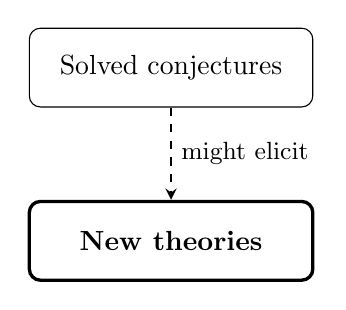
\begin{tikzpicture}[box/.style={draw, rounded corners, align=center, minimum height=1cm, minimum width=3.6cm}, >=stealth]
\node[box] (a) at (0,2.2) {Solved conjectures};
\node[box, very thick] (b) at (0,0) {\textbf{New theories}};
\draw[->, thick, dashed] (a) -- node[right] {\small might elicit} (b);
\end{tikzpicture}

\vspace{0.6em}
The goal is understanding
\column{0.46\textwidth}
\centering
\onslide<2->{
\textbf{ML}

\vspace{0.6em}
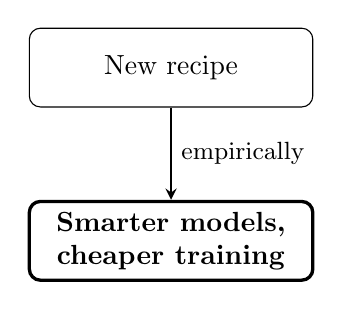
\begin{tikzpicture}[box/.style={draw, rounded corners, align=center, minimum height=1cm, minimum width=3.6cm}, >=stealth]
\node[box] (a) at (0,2.2) {New recipe};
\node[box, very thick] (b) at (0,0) {\textbf{Smarter models,}\\\textbf{cheaper training}};
\draw[->, thick] (a) -- node[right] {\small empirically} (b);
\end{tikzpicture}

\vspace{0.6em}
The goal is whatever works
}
\end{columns}
\vspace{1.2em}
\centering
\onslide<3->{``The equivalent of grinding through random conjectures would be enormously valuable in machine learning in a way that it just isn't in mathematics.''}
\source{patel2026}
\end{frame}

\begin{frame}{Even the Transformer Was a Combination of Known Pieces}
\centering
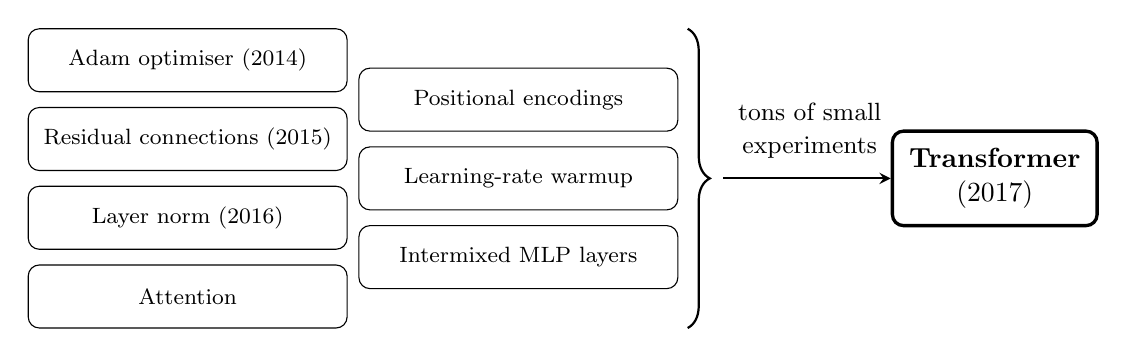
\begin{tikzpicture}[piece/.style={draw, rounded corners, align=center, minimum height=0.8cm, minimum width=4.05cm, font=\footnotesize}, >=stealth]
\node[piece] (p1) at (0,3.0) {Adam optimiser (2014)};
\node[piece] (p2) at (0,2.0) {Residual connections (2015)};
\node[piece] (p3) at (0,1.0) {Layer norm (2016)};
\node[piece] (p4) at (0,0) {Attention};
\node[piece] (p5) at (4.2,2.5) {Positional encodings};
\node[piece] (p6) at (4.2,1.5) {Learning-rate warmup};
\node[piece] (p7) at (4.2,0.5) {Intermixed MLP layers};
\onslide<2->{
\draw[decorate, decoration={brace, amplitude=8pt}, thick] (6.35,3.4) -- (6.35,-0.4);
\node[draw, rounded corners, very thick, align=center, minimum height=1.2cm, minimum width=2.6cm] (t) at (10.25,1.5) {\textbf{Transformer}\\(2017)};
\draw[->, thick] (6.8,1.5) -- (t);
\node[align=center] at (7.9,2.1) {\small tons of small\\\small experiments};
}
\end{tikzpicture}

\vspace{1.2em}
\onslide<3->{Persistently matching combinations of known ideas:\\exactly what AIs are disproportionately good at in maths}
\source{patel2026}
\end{frame}

\begin{frame}{AI R\&D Is Largely Verifiable}
\begin{columns}[t]
\column{0.32\textwidth}
\centering
{\Large\faBook}

\textbf{Pretraining}

\vspace{0.4em}
\raggedright\small
\begin{itemize}
\item Loss on a held-out test set
\item Compute to reach a fixed loss
\item ``Taste-bench'': will a gain at 100M parameters hold at 10B?
\end{itemize}
\column{0.32\textwidth}
\centering
\onslide<2->{
{\Large\faDumbbell}

\textbf{Post-training}

\vspace{0.4em}
\raggedright\small
\begin{itemize}
\item Compute, data or time to train on new environments
\item How fast a model learns an environment it has never seen
\item Redoing real problems lab researchers solved
\end{itemize}
}
\column{0.32\textwidth}
\centering
\onslide<3->{
{\Large\faTachometer*}

\textbf{Inference efficiency}

\vspace{0.4em}
\raggedright\small
\begin{itemize}
\item GPU utilisation
\item KV cache size per token
\item FLOPs in a forward pass
\item Latency
\end{itemize}
}
\end{columns}
\vspace{1.6em}
\centering
\onslide<4->{``AI training is literally happening inside a datacenter.''}
\source{patel2026}
\end{frame}

\begin{frame}{Explicit Modelling}
\centering
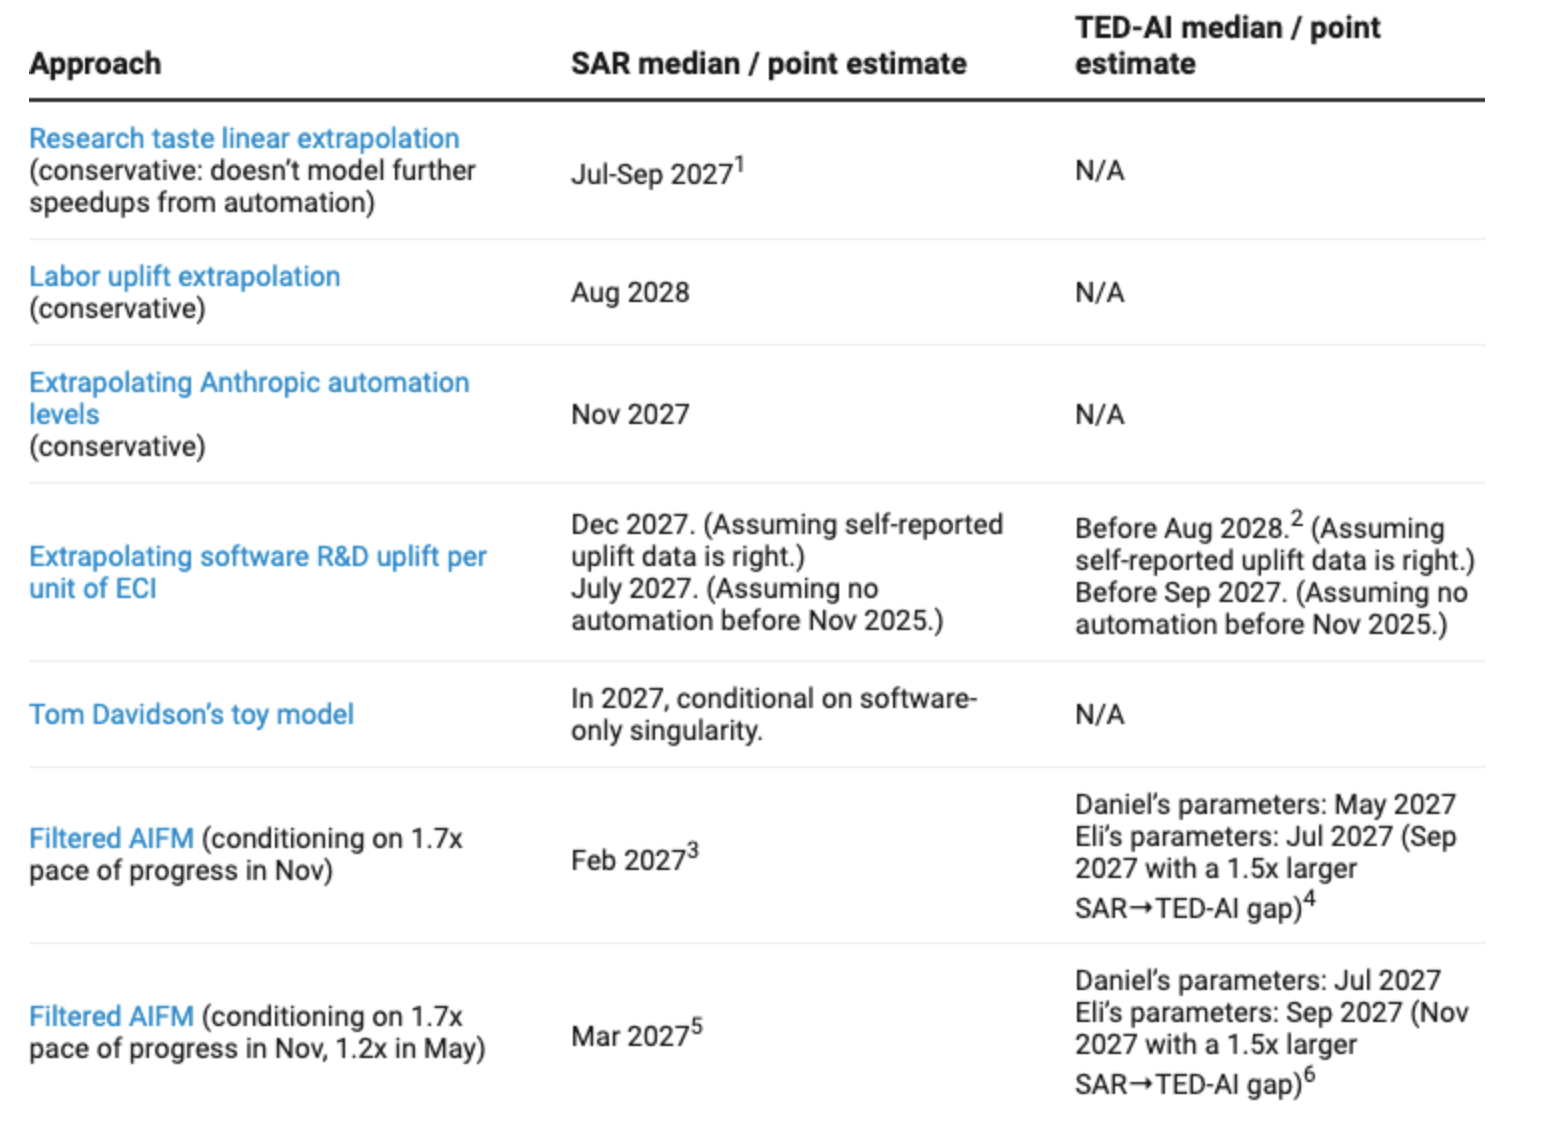
\includegraphics[height=0.74\textheight]{bib/lifland2026/figures/methods_forecast}
\source{lifland2026}
\end{frame}

\begin{frame}{AI 2027: Where Are We in the Scenario?}
\centering
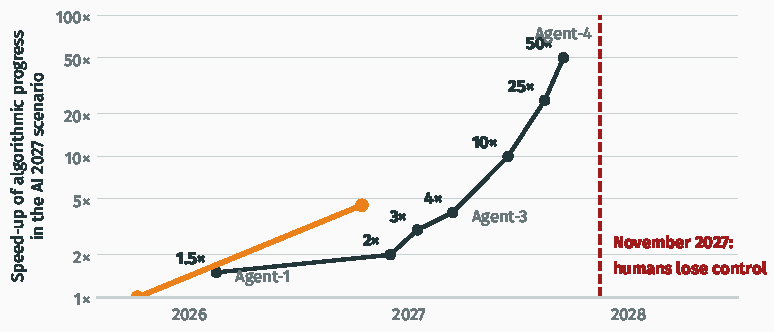
\includegraphics[width=\textwidth]{ai2027_speedup}
\source{kokotajlo2025a,metr2026}
\end{frame}
